% Chapter 2

\chapter{Literature Review} %chapter title

\label{Chapter2} % For referencing  use \ref{Chapter2} 

Summarizing and analyzing existing research, studies, and relevant
publications that relate to our project.

\section{Market Trends in India}
\subsection{Real Estate Market Trends}
\begin{enumerate}
      \item \textbf{Urbanization and Population Growth:} India's rapid urbanization
            continues to drive demand for housing. With a growing population
            and increasing urban migration, the need for affordable and
            accessible housing remains a significant trend.~\cite{urbanization-and-its-impact-on-housing}
      \item \textbf{Shift in Rental Preferences:} There has been a shift in preferences
            among the younger population towards rental accommodations
            due to mobility for jobs, lower commitment, and financial
            flexibility. This shift is particularly notable in metro cities
            and urban hubs.
      \item \textbf{Co-living and Co-working Spaces:} Emerging trends show a rise in
            demand for co-living spaces and co-working environments, especially
            among millennials and young professionals. These spaces offer a sense of
            community, shared amenities, and cost-effectiveness.\par
            The rise of co-living and co-working spaces is not just a trend; it's a
            significant shift in urban lifestyles. In densely populated cities like
            Mumbai, Delhi, and Bengaluru, these concepts are addressing the challenges
            of affordable housing and the need for flexible, productive workspaces.
            Moreover, co-living offers attractive returns—2-4 times higher than the
            traditional residential yield of 2-3 per cent—leading to higher investors’ i
            nterest in actively pursuing options in the market to create flexible
            co-living facilities.~\cite{investors-on-coliving}
      \item \textbf{Tech Integration in Real Estate:} Technology adoption in real estate
            has seen substantial growth. Digital platforms for property searches,
            virtual property tours, and online rent payment systems have gained
            popularity, enhancing convenience for both landlords and tenants.
      \item \textbf{Government Initiatives:} Various government initiatives like the
            Pradhan Mantri Awas Yojana (PMAY) and Smart Cities Mission aim to
            provide affordable housing and improve infrastructure, influencing the
            real estate landscape and rental market dynamics.
\end{enumerate}

\subsection{Rental Market Trends}
\begin{enumerate}
      \item \textbf{Rise in Rental Yields:} Despite fluctuations, rental yields have been stable or
            rising in certain areas, attracting investors and encouraging property owners to
            engage in the rental market.
      \item \textbf{Demand for Flexible Rentals:} There's an increasing demand for flexible rental options,
            including short-term leases and furnished accommodations, particularly from young professionals
            and students.
      \item \textbf{Emergence of PropTech Solutions:} Proptech startups are introducing innovative solutions for
            property management, tenant screening, and rent collection, streamlining processes for both landlords
            and tenants.
      \item \textbf{Localized Rental Dynamics:} Rental markets vary significantly across different cities and regions
            in India. For instance, metropolitan areas like Mumbai and Delhi exhibit different rental patterns,
            pricing structures, and demand-supply dynamics compared to tier-II or tier-III cities.
      \item \textbf{Rental Regulations and Policies:} Rental laws and regulations, such as the Rent Control Act and
            local tenancy laws, significantly impact the rental market. Understanding these regulations is crucial
            for both landlords and tenants.~\cite{public-social-rental-housing-in-india}
\end{enumerate}

\bigskip
\subsection{Recent Developments and Future Projections}
\begin{enumerate}
      \item \textbf{Post-Pandemic Impact:} The COVID-19 pandemic has influenced the rental market, causing temporary shifts
            like increased demand for spacious homes, a surge in remote work leading to altered location preferences, and a
            focus on hygiene and safety in rental spaces.
      \item \textbf{Technology and Data Analytics:} Continued integration of technology, including AI-driven property searches,
            blockchain for secure transactions, and data analytics for market predictions, is expected to redefine the rental
            landscape, making it more efficient and transparent.
      \item \textbf{Sustainability and Green Spaces:} Growing awareness of sustainability and environmental concerns is
            influencing rental choices, with preferences for eco-friendly properties and communities on the rise.
      \item \textbf{Policy Changes:} Anticipated policy changes or amendments in rental laws, especially concerning tenancy
            agreements and rent control, could significantly impact the market dynamics in the coming years.
\end{enumerate}

\section{Why we chose the PropTech sector?}
The story of proptech startups in India took shape in the mid-2000s after the entry of Info Edge-owned
99acres and Times Internet-owned Magicbricks, Quikr-owned CommonFloor and PropTiger (REA India)-owned Makaan.com.
Following this, the story revolved around Housing.com, a once-celebrated startup which then faced a series of mishaps.
In the past five years, the proptech segment has evolved manifold and has seen startups in brokerage tech led by
Square Yards, construction tech led by Infra.Market, AI, AR, VR, IoT, SaaS, and other spaces.

\clearpage
\begin{wrapfigure}{r}{0.5\textwidth}
      \centering
      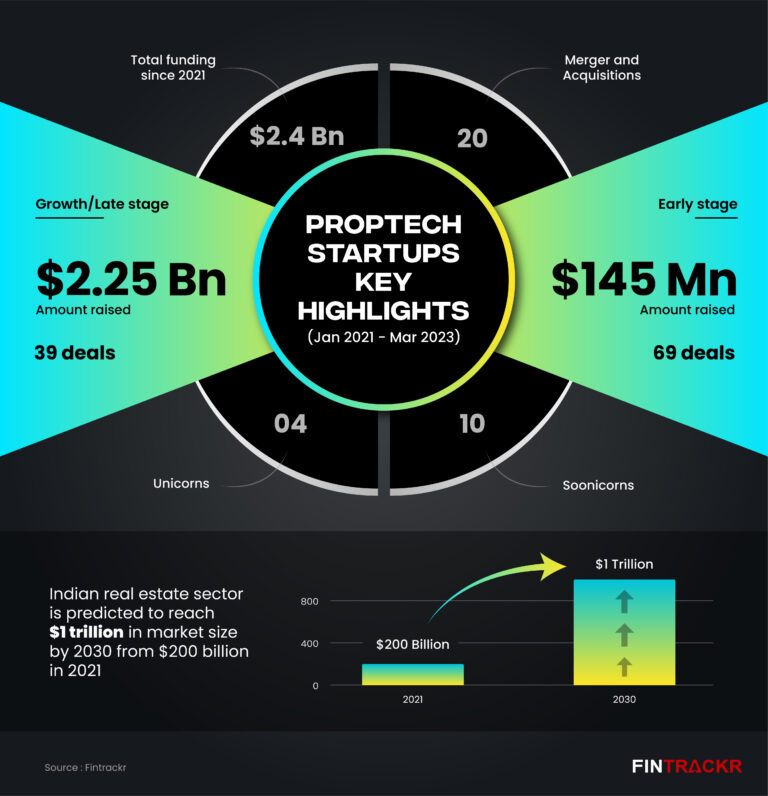
\includegraphics[width=0.48\textwidth]{Images/proptech1.jpg}
      \caption{Key Highlights}
\end{wrapfigure}

The Indian real estate sector is predicted to reach \$1 trillion in market size by 2030, up from \$200 billion in 2021,
and contribute to 13\% of the country’s GDP by 2025.  And looks like tech companies in this space have a role to play as
well. As per data compiled by Fintrackr, proptech startups have mopped up nearly \$2.4 billion between January 2021 and
March 2023. This comprises 39 growth stage companies raising \$2.25 billion and 69 early stage startups raising \$145 million.
If we take previous data, then proptech startups have managed to raise \$2.9 billion since January 2020.\par
\smallskip

Funding in proptech startups peaked in 2018 with \$1.28 billion. Even as the trend continued in 2019, the impact of lockdown
can be seen in 2020 when the fundraise plunged to less than \$500 million. This again saw a revival in 2021,
only soon to get impacted by an overall slowdown in the funding environment in 2022 and 2023. While pre-Covid era was
dominated by the likes of OYO, co-working space providers, the post-Covid period saw massive funding in construction
and building material focused startup such as Infra.Market, real estate rental startup NoBroker, home decor and interior
startups Livspace and HomeLane.~\cite{growth-of-proptech-post-covid}\par

\begin{figure}[h]
      \centering
      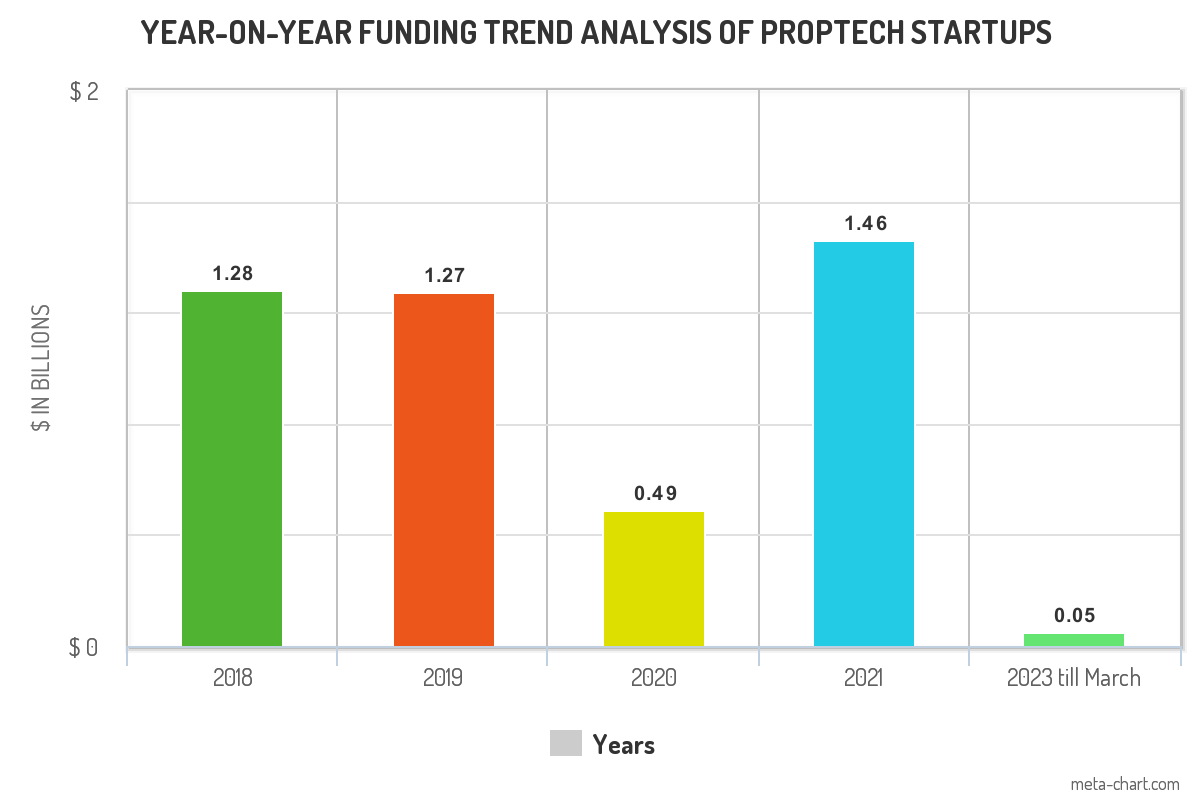
\includegraphics[width=0.7\textwidth]{Images/meta-chart.png}
      \caption{Funding trend analysis}
\end{figure}

In this section, we have highlighted top funded startups in proptech and their capital efficiency ratio based on their
financial performance in FY22.\par\medskip

\begin{table}[h]
      \centering
      \caption{Capital Efficiency of top PropTech Startups}
      \begin{tabular}{llll}
            \toprule
            Name          & Revenue(FY22)   & Overall Funding & Capital Efficiency \\
            \midrule
            IndiQube      & \rupee 6236 Cr  & \rupee 342 Cr   & 2.00               \\
            WeWork India  & \rupee 351.4 Cr & \rupee 1300 Cr  & 1.03               \\
            Awfis         & \rupee 257 Cr   & \rupee 760 Cr   & 0.50               \\
            NestAway      & \rupee 57.8 Cr  & \rupee 828 Cr   & 0.07               \\
            Stanza Living & \rupee 115 Cr   & \rupee 1672 Cr  & 0.07               \\
            NoBroker      & \rupee 116 Cr   & \rupee 2743 Cr  & 0.06               \\
            \bottomrule
      \end{tabular}
\end{table}

\begin{table}[h]
      \centering
      \caption{Top Revenue Generating Real Estate Focused Companies}
      \begin{tabularx}{\textwidth}{XX}
            \toprule
            Name         & Revenue(FY21)   \\
            \midrule
            Square Yards & \rupee 245.7 Cr \\
            Anarock      & \rupee 182 Cr   \\
            99acres      & \rupee 173.8 Cr \\
            Housing.com  & \rupee 88 Cr    \\
            PropTiger    & \rupee 50.57 Cr \\
            NoBroker     & \rupee 166.5 Cr \\
            Quikr Homes  & \rupee 60.7 Cr  \\
            MagicBricks  & \rupee 166 Cr   \\
            \bottomrule
      \end{tabularx}
\end{table}

\clearpage
\section{Co-Living \& Renting Together}

We live in a globally connected world and this has led to the real estate sector
experiencing disruption led by nomadic millennials, who are redefining the meaning
of ‘living’ and ‘working’. The concept of ‘shared economy’ has just started to
unfold in India and the days ahead look much more exciting. Unlike earlier when ‘ownership’
was fundamental to success in life, today ‘sharing’ has taken the centre stage.\par

\subsection{Framework of Analysis}
JLL Research conducted a comprehensive demand survey targeting millennials across
the top seven cities of Mumbai, Delhi NCR, Bengaluru, Hyderabad, Chennai, Kolkata
and Pune. The key objective of this assessment was to study their behavioural patterns
for owning and renting houses.\par\medskip
\begin{wrapfigure}{r}{0.5\textwidth}
      \centering
      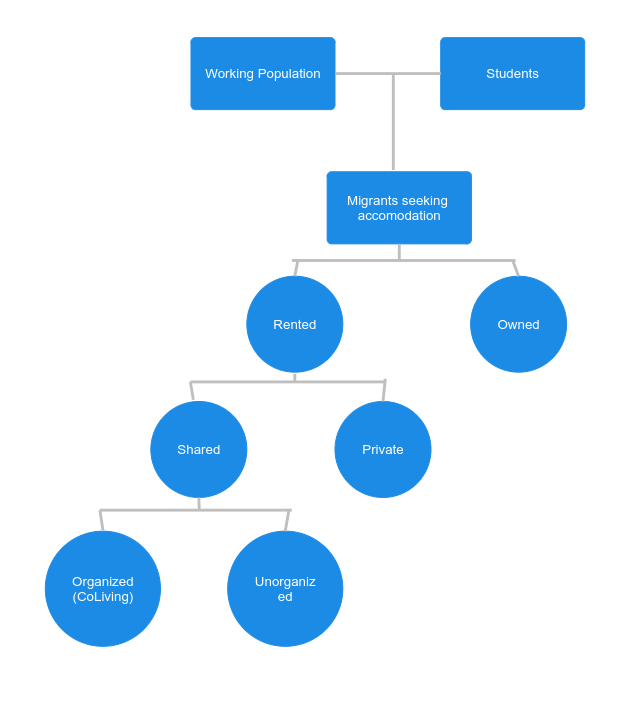
\includegraphics[width=0.48\textwidth]{Images/framework.png}
      \caption{Framework Analysis}
\end{wrapfigure}
The nomads of today are becoming a major force driving the Indian housing market—an estimated 42% of the workforce in India
constituted millennials1 in 2018 across the top seven cities in India. It is relevant to note that millennials will continue to form a major
proportion of the country’s working population, growing to nearly 41\% of the workforce in 2023.
\textbf{\textit{Nearly 40\% of India’s millennial workforce are migrants}}\par

\subsubsection{Migrant millenial workforce prefers to rent}
With millennials driving housing demand, there is a marked change in demand patterns. Gen Y has a different take on home
ownership from their parents. Earlier generations moved to the peripheral locations to fulfil their dreams of owning a home, but
millennials refuse to compromise.\par\medskip
While selecting an accommodation, connectivity to their workplace, convenience and security are the factors on top of their
decision making tree and not ownership of the property. Moreover, a migrant workforce prefers rented apartments because of the
uncertainty attached with the duration of their stay as well as cost savings in renting as against purchasing accommodation.\par\medskip
The outcome-an increased demand for rental housing.

\subsection{Owning vs Renting a house}
\noindent Home ownership has been long considered as a basis to measure financial and social security in India.
However, there has been a discernible change in the mind-set and the behaviour of the recent generations. This is attributable to the following:\par

\begin{enumerate}
      \item High cost of housing in most gateway cities and lower returns from buying a house (EMI to rent ratio is typically 2-3 times in
            most cities).
      \item Change in the nature of work - short term nature of assignments warranting higher mobility and flexibility.
      \item Delayed marriage and child rearing, less inclination to block funds and rather spend on travel, food and leisure (considered to
            be discretionary in the past).
\end{enumerate}

\begin{itemize}
      \item 93\% of the migrant respondents who were single stayed in rented accommodation across the top 7 cities
      \item 60\% said that they didn’t plan or were unsure about buying a house in the future
      \item Budget constraints and limited flexibility were cited as the key reasons for not owning a house
\end{itemize}

\clearpage
\begin{figure}[h]
      \centering
      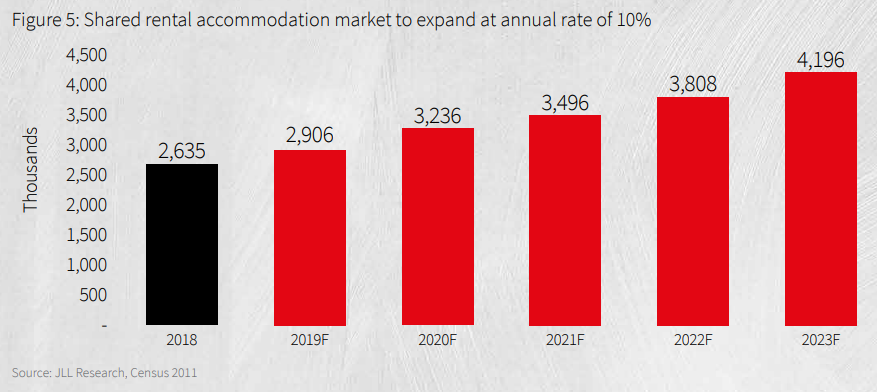
\includegraphics[width=1\textwidth]{Images/shared_market_trends.png}
      \caption{Funding trend analysis}
\end{figure}

\begin{wrapfigure}{l}{0.4\textwidth}
      \centering
      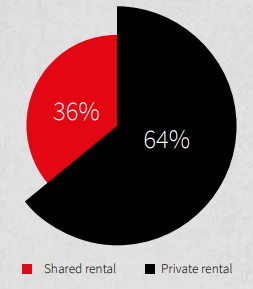
\includegraphics[width=0.35\textwidth]{Images/shared_pref.png}
      \caption{Living Preferences}
\end{wrapfigure}

Here's Why Milennials Find Shared Rental Apartments Most Vaiable:
\begin{itemize}
      \item Cities like Delhi, Pune, Hyderabad, Bengaluru, Mumbai, Chennai and Kolkata attract
            millennials for education as well as employment
      \item  Millennials consider proximity to workplace or education institute as most important while
            choosing accommodation
      \item Renting private apartment in commercial or educational hub beyond financial means of
            most millennials
      \item With housing rent typically accounting for 25-30\% of average monthly income in urban
            India, rental costs get apportioned in case of shared accommodation~\cite{coliving-reshaping-rental-housing-in-india}
\end{itemize}
